\section{Rešitev}
\subsection{Obvezen del}
Najprej rešitev s furjerjem = neumanov r.p.
\begin{figure}[h]
    \centering
    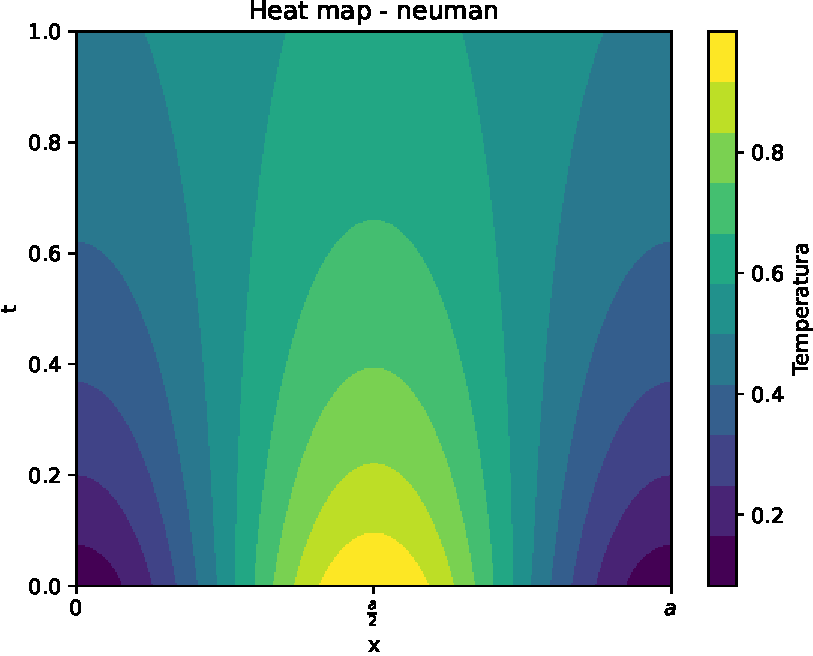
\includegraphics[width=0.7\textwidth]{pdfs/heat_map.pdf}
    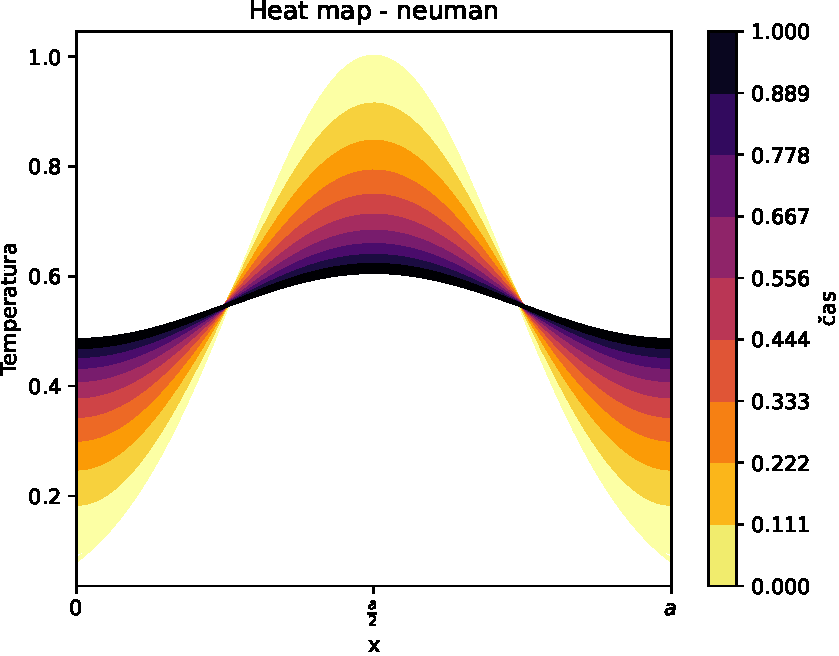
\includegraphics[width=0.7\textwidth]{pdfs/heat_map2.pdf}
    \caption{Neumanov robni pogoj - fft metoda}
\end{figure}
Za ta primier imam tudi animacijo (precej generericna) v datoteki animations

\newpage
\begin{figure}[h]
    \centering
    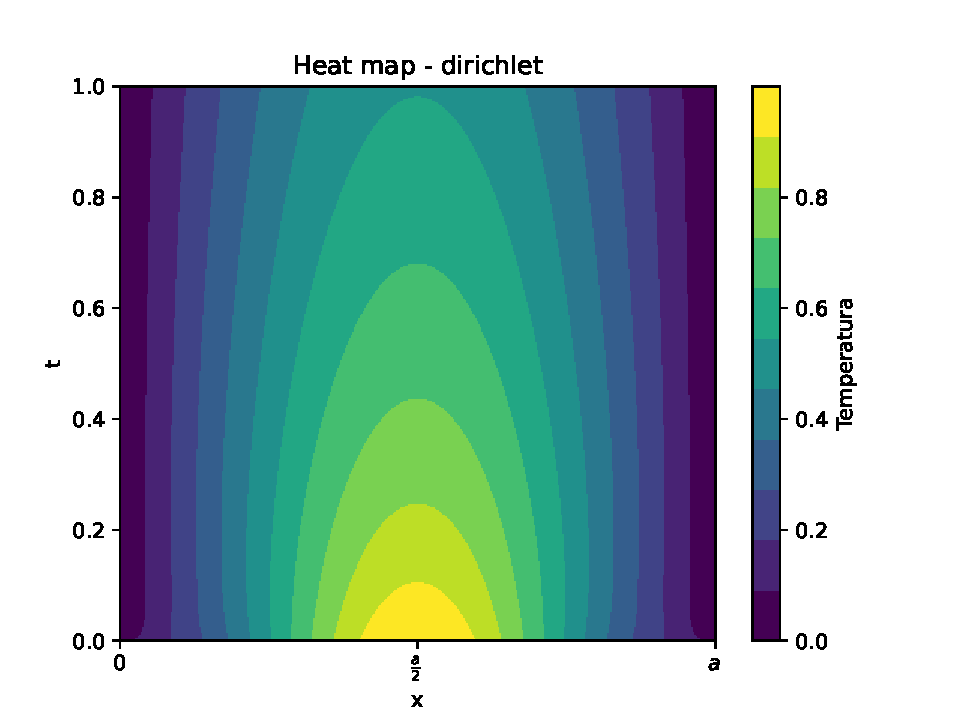
\includegraphics[width=0.7\textwidth]{pdfs/heat_map_direchlet.pdf}
    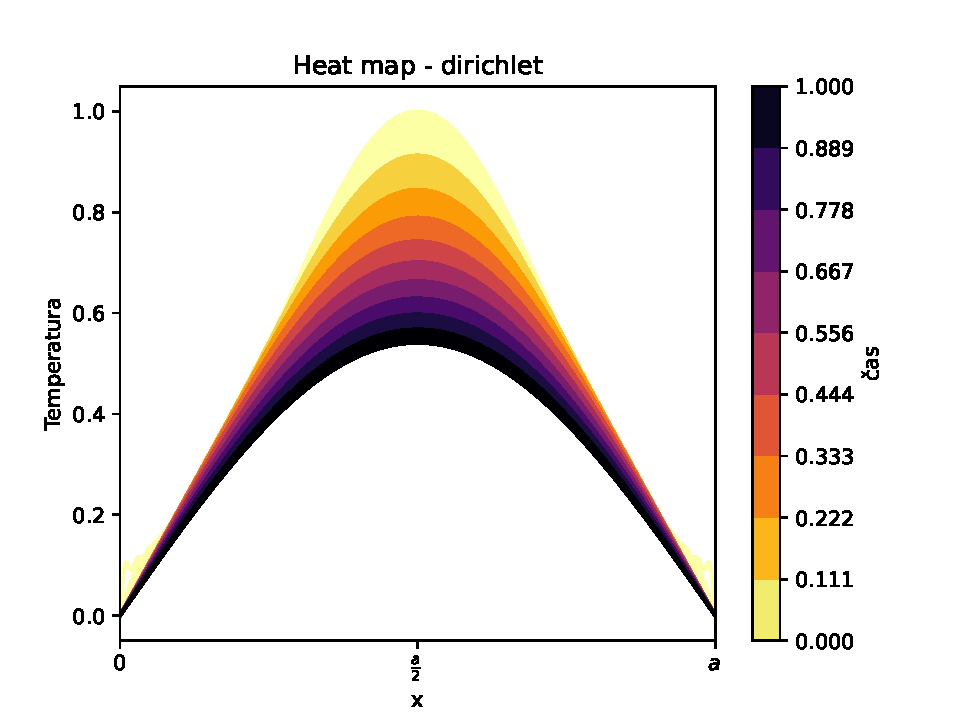
\includegraphics[width=0.7\textwidth]{pdfs/heat_map2_direchlet.pdf}
    \caption{Dirichletov robni pogoj - skalarni produkt}
\end{figure}

\newpage
Poglejmo še zlepke, najpočasnejša metoda in najbolj nenatančna.
\begin{figure}[h]
    \centering
    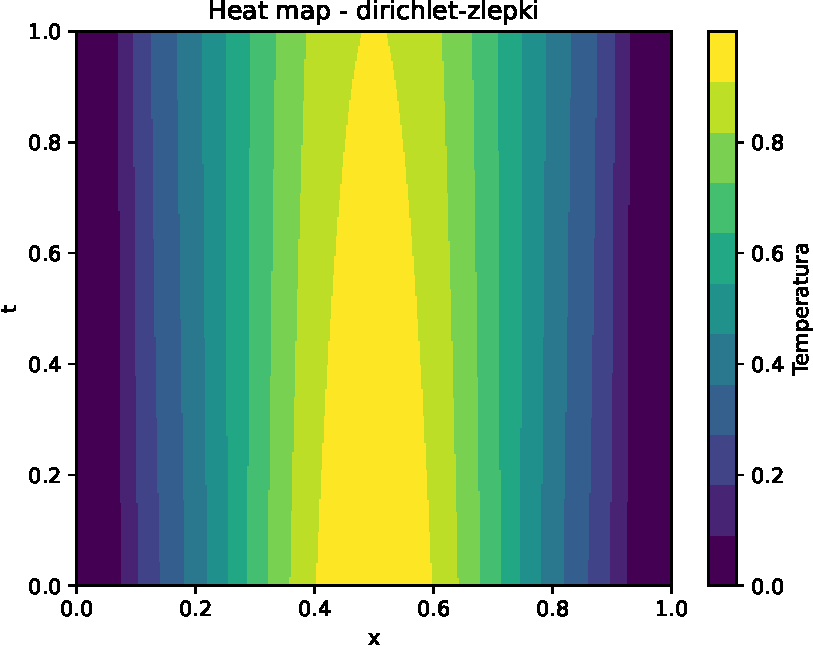
\includegraphics[width=0.6\textwidth]{pdfs/zlepki.pdf}
    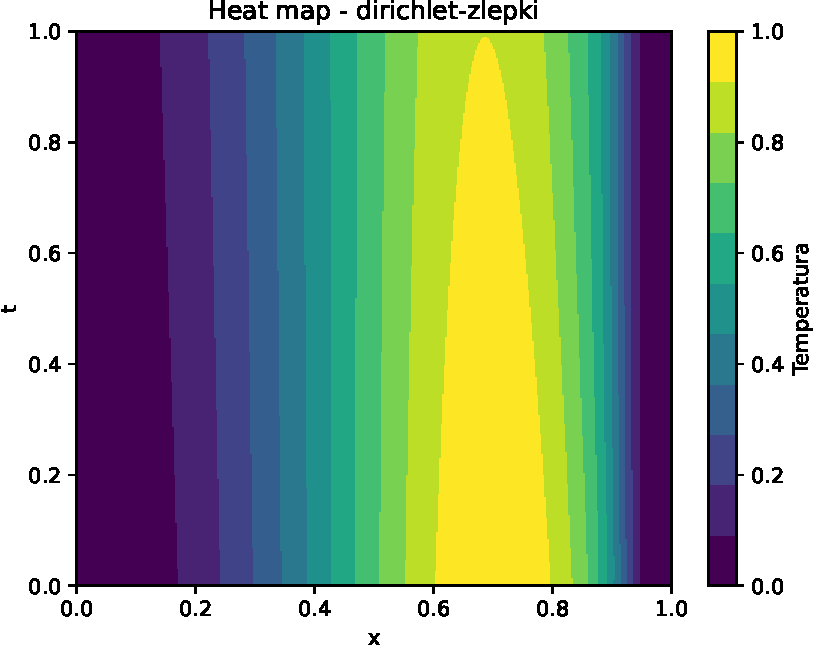
\includegraphics[width=0.6\textwidth]{pdfs/zlepki2.pdf}
    \caption{Dirichletov robni pogoj z metodo zlepkov. 
    Prva slika je za začeteno temperaturo obliki gavsovke, druga pa ima obliko $\sin(\pi x^2)$}
\end{figure}
\newpage
\subsection{Dodaten del}
\begin{figure}[h]
    \centering
    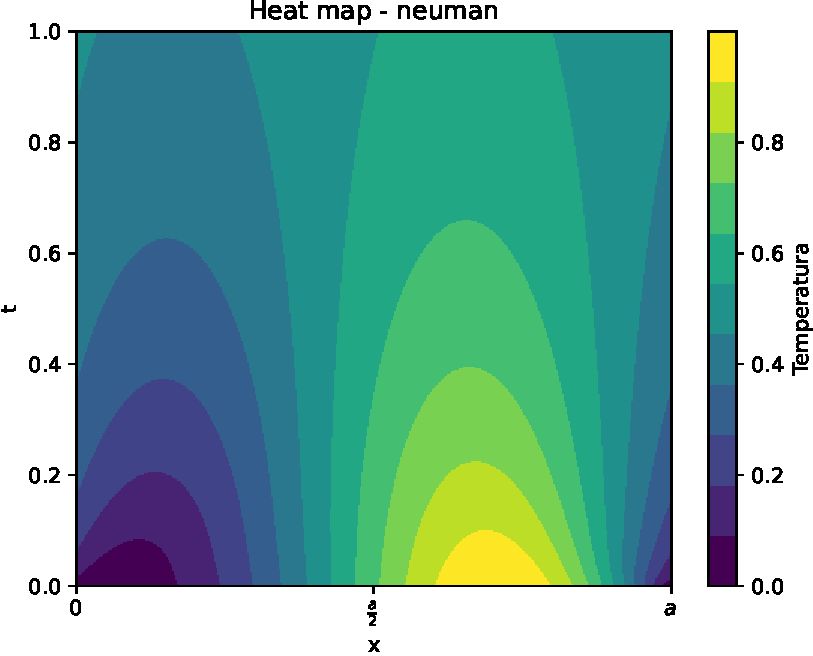
\includegraphics[width=0.7\textwidth]{pdfs/heat_map-neuman.pdf}
    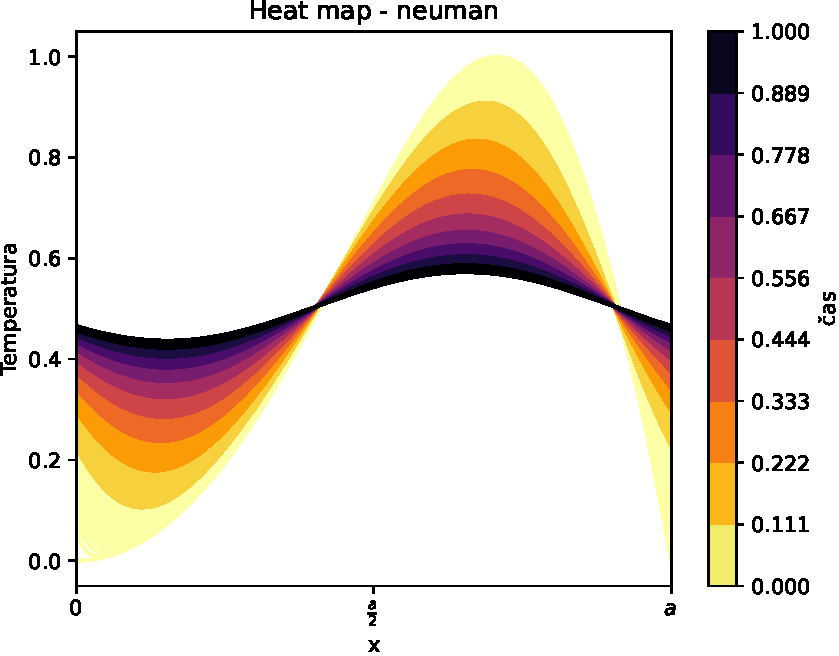
\includegraphics[width=0.7\textwidth]{pdfs/heat_map-neuman2.pdf}
    \caption{Neumanov robni pogoj z fft metodo za začeten temperaturni profil
    $\sin(\pi x^2)$}
\end{figure}
\newpage
\begin{figure}[h]
    \centering
    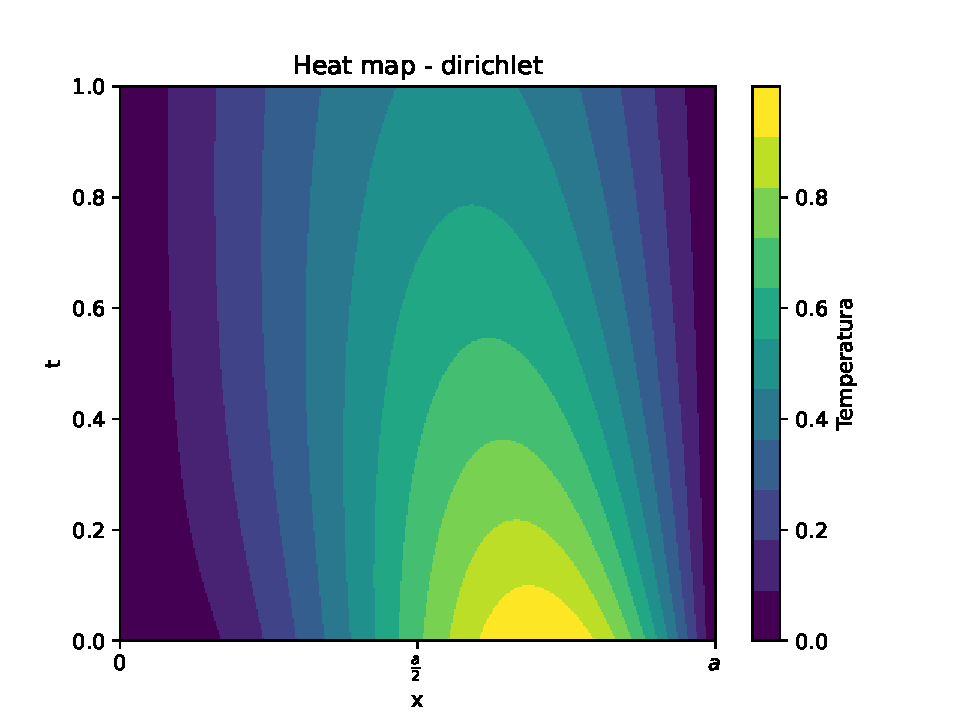
\includegraphics[width=0.7\textwidth]{pdfs/heat_map_direchlet2.pdf}
    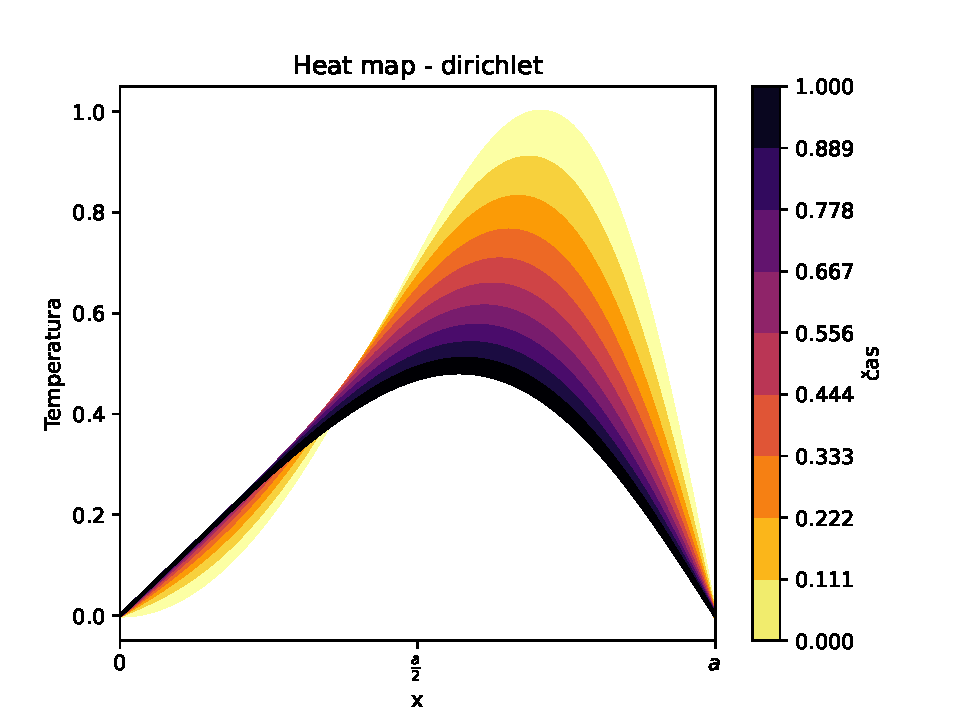
\includegraphics[width=0.7\textwidth]{pdfs/heat_map2_direchlet2.pdf}
    \caption{Dirichletov robni pogoj s skalarnim produtkom in z začetnim temperaturnim profilom
    $\sin(\pi x^2)$}
\end{figure}
